\documentclass{beamer}
\setbeamertemplate{navigation symbols}{}
\usepackage{xcolor}
\definecolor{seeblau}{HTML}{00A9E0}
\definecolor{seegrau}{HTML}{9AA0A7}

\definecolor{seeblau1}{HTML}{CCEEF9}
\definecolor{seeblau2}{HTML}{A6E1F4}
\definecolor{seeblau3}{HTML}{59C7EB}
\definecolor{seeblau4}{HTML}{00A9E0}
\definecolor{seeblau5}{HTML}{008ECE}

\setbeamercolor{title}{fg=seeblau}
\setbeamercolor{frametitle}{fg=seeblau}
\setbeamercolor{section in toc}{fg=seeblau}
\setbeamercolor{structure}{fg=seeblau}

\setbeamertemplate{footline}{%
	\begin{beamercolorbox}[sep=.25cm,wd=\paperwidth,leftskip=0.25cm,rightskip=0.25cm]{footlinecolor}
		\small
		% \textbf{\insertsection}\quad\insertsubsection
		% \hfill\insertframenumber
	\end{beamercolorbox}%
}

\usepackage[overridenote]{pdfpc}

\usepackage[english]{babel}
\parskip=20pt

\usepackage[sfdefault]{roboto}
\usepackage{libertinust1math}
\usefonttheme[onlymath]{serif}

\usepackage{ifthen, adjustbox}
\newcommand{\markieren}[4]{
	\ifthenelse{\equal{#1}{}}{}{\adjustbox{padding=3pt, bgcolor=seeblau1, margin=-1pt}{\strut{\sffamily\robotoMedium{#1}}}\\}
  \ifthenelse{\equal{#2}{}}{}{\adjustbox{padding=3pt, bgcolor=seeblau2, margin=-1pt}{\strut{\sffamily\robotoMedium{#2}}}\\}
	\ifthenelse{\equal{#3}{}}{}{\adjustbox{padding=3pt, bgcolor=seeblau3, margin=-1pt}{\strut{\sffamily\robotoMedium{#3}}}\\}
	\ifthenelse{\equal{#4}{}}{}{\adjustbox{padding=3pt, bgcolor=seeblau4, margin=-1pt}{\strut{\sffamily\robotoMedium{#4}}}}
}

\let\footnoterule\relax % removes bar
\setbeamertemplate{footnote}{
  \parindent 0em\noindent
  \raggedleft
  \usebeamercolor{footnote}\hbox to 0.8em{\hfil\insertfootnotemark}\tiny\insertfootnotetext\par%
}

\newcommand\blfootnote[1]{
	\let\thefootnote\relax\footnotetext{#1}
}

\usepackage[
	style=authortitle
]{biblatex}
\usepackage{ifthen}
\newcommand{\customcite}[2][]{
	\blfootnote{
		\emph{\citetitle{#2}}, \citeauthor*{#2} \citeyear{#2}
		\ifthenelse{ \equal{#1}{} }{}{(#1)}
	}
}


\usepackage[ddmmyyyy]{datetime}
\renewcommand{\dateseparator}{.}

\usepackage{amsmath,amssymb,amsfonts,amsthm}

\addbibresource{literature.bib} 

\title{Noise Analysis in an Optomechanical Resonance Cavity}
\author{Leon Oleschko}
\institute{Universität Konstanz}
\date{\today}

\begin{document}
{
\setbeamertemplate{footline}{} 
\begin{frame}
	\huge
	\markieren{}{}{Noise Analysis}{Optomechanical Cavity}
	
	\vfill
	\normalsize
	Leon Oleschko\\
	\today
	
	\vfill
	\raggedleft
	\small
	\textit{Modeling Quantum Hardware: open dynamics and control}\\
	Universität Konstanz
\end{frame}
}

\section{Problem Statement}
\begin{frame}{Problem Statement}
	\begin{columns}
		\column{0.5\textwidth}
		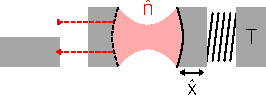
\includegraphics[width=\textwidth]{figures/drawing.pdf}

	\end{columns}

	\customcite{aspelmeyer_cavity_2014}
	\customcite{bowen_quantum_2015}
\end{frame}

\begin{frame}{Hamiltonian}

	{
		\small
		Optical Cavity $\hat a$, $\omega_o(\hat x_\text{mech}) = \omega_o + \frac{g}{\omega_o} \hat x_\text{mech}$;
		mechanical oscillations $\hat b, \omega_m$;
		coupling $g$;
		Drive $E$, $\omega_L$
		\blfootnote{$\hbar=1$}
	}
	$$
		H = \underbrace{
			\omega_o\; a^\dagger a
		}_\text{Cavity} 
		+ \underbrace{
			\omega_m\; b^\dagger b
		}_\text{Mechanical}
		- \underbrace{
			g\; a^\dagger a\; (b + b^\dagger)
		}_{\text{Interaction}}
		+ \underbrace{
			E ( a e^{i\omega_L t} + a^\dagger e^{-i\omega_L t} )
		}_{\text{Drive}}
	$$

	\pause
	\emph{Rotating Wave Approximation} at $\omega_L$ with $\Delta = \omega_o - \omega_L$, $a \rightarrow ae^{i\omega_L t}$:
	$$
		H_\text{RWA} = \Delta\; a^\dagger a + \omega_m\; b^\dagger b - g\; a^\dagger a\; (b^\dagger + b) + E ( a + a^\dagger)
	$$

	\customcite[2.3]{bowen_quantum_2015}
	\customcite[Optomechanical Cavity]{noauthor_quantumopticsjl_nodate}
\end{frame}

\begin{frame}{Hamiltonian Linearization}
	{
		\color{seegrau}
		$$
			H_\text{RWA} = \Delta\; a^\dagger a + \omega_m\; b^\dagger b - g\; a^\dagger a\; (b^\dagger + b) + E (a+ a^\dagger)
		$$
	}	

	Linearize $a = \alpha + \delta a$, $b = \beta + \delta b$; with $\alpha, \beta$ steady state.\\
	\begin{align*}
		H_\text{Interaction} &= 
		- g\; a^\dagger a\; (b^\dagger + b)\\
		&\approx -\underbrace{g |\alpha|}_{G} 
		\left(\delta a + \delta a^\dagger + {\color{seegrau}\mathcal{O}(a^2 + \delta a \delta a^\dagger) }\right)
		\left(\delta b + \delta b^\dagger + {\color{seegrau} 2 \beta}\right)
	\end{align*}

	\pause
	Therefore for small $G$:
	$$
	H \approx \Delta\; \delta a^\dagger \delta a 
	+ \omega_m \delta b^\dagger \delta b
	- G (\delta a + \delta a^\dagger)(\delta b + \delta b^\dagger)
	$$

	\customcite[2.7]{bowen_quantum_2015}
\end{frame}

\begin{frame}{Dissipation}
	Optical decay $\kappa$:
	$$J_O = \sqrt{\kappa} \; \delta a$$
	
	Mechanical resonator with $\gamma$ and a thermal bath at the $n$-th thermal state:
	$$
		J_M = 
		\sqrt{\gamma (n+1)} \;\delta b 
		+ \sqrt{\gamma n} \; \delta b^\dagger
	$$
	\customcite[2.8]{bowen_quantum_2015}
\end{frame}

\section{Implementation}
\begin{frame}{Implementation}
\begin{enumerate}
	\item truncated Fock Basis: $F_\text{optical} \otimes F_\text{mechanical}$
	\item definition of $H, J$ with $\delta a \otimes 1$
	\item Master Time Evolution: 
	$$
		\dot\rho = -i[H,\rho] + J\rho J^\dagger - \frac{1}{2} J^\dagger J \rho - \frac{1}{2}\rho J^\dagger J
	$$
\end{enumerate}
\customcite{noauthor_quantumopticsjl_nodate}
\end{frame}

\begin{frame}{Time evolution}
	\centering
	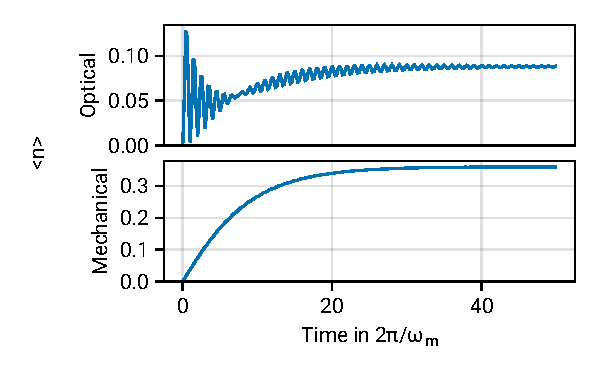
\includegraphics{figures/02 time evolution.pdf}
\end{frame}


{
	\setbeamercolor{background canvas}{bg=black}
	\begin{frame}[plain]{}\end{frame}
}

\end{document}